\section{\texorpdfstring{Realizace logického obvodu}{Realizace logickeho obvodu}}

% =====================================================================================================================
	\begin{frame}
    \frametitle{Prvky logického obvodu - hradla}
		\boldmath
		\small
		
		\begin{minipage}[t][\textheight][t]{0.5\textwidth}
		\vspace{5mm}
		\begin{center}
			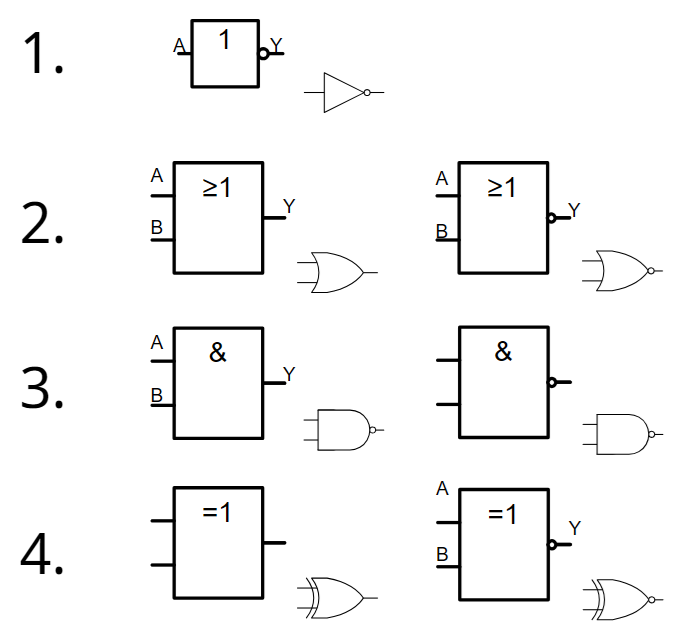
\includegraphics[width=\textwidth]{fig/hradla.png}
		\end{center}

		\end{minipage}
		\begin{minipage}[t][\textheight][t]{0.45\textwidth}
    \vspace{5mm}

			\begin{enumerate}
				\item Invertor - negace \\ $Y = \bar{A}$ \\ \vspace{3mm}
				\item OR, NOR \\ $Y = A + B$ \\ $Y = \overline{A + B}$ \\ \vspace{3mm}
				\item AND, NAND \\ $Y = A \cdot B$ \\ $Y = \overline{A \cdot B}$ \\ \vspace{3mm}
				\item XOR, XNOR \\ $Y = A \bar{B} + \bar{A}B$ \\ $Y = \bar{A}\bar{B} + AB$ \\ \vspace{3mm}
			\end{enumerate}
    
		\end{minipage}
		
	\end{frame}
	
% =====================================================================================================================
	\begin{frame}
    \frametitle{Neekvivalence a ekvivalence - hradlo XOR a XNOR}
		\boldmath
		
		\begin{itemize}
			\item Zjednodušuje obvody sčítaček, výpočtu parity, porovnávání apod.
			\item Obtížně se určuje z Karnaughovy mapy.
			\item Lze jej nahradit logickým obvodem s hradly AND, OR, NEG.
		\end{itemize}
		
		\begin{minipage}[t][\textheight][t]{0.5\textwidth}
		\vspace{5mm}
		\begin{center}
			\includegraphics[scale=0.3]{fig/xor.png}
			
			\begin{tabular}{ c c | c}
				A & B & Y \\
				\hline
				0 & 0 & 0 \\
				0 & 1 & 1 \\
				1 & 0 & 1 \\
				1 & 1 & 0 \\
			\end{tabular}
		\end{center}

		\end{minipage}
		\begin{minipage}[t][\textheight][t]{0.45\textwidth}
    \vspace{5mm}
		\begin{center}
			\includegraphics[scale=0.3]{fig/xnor.png}
			
			\begin{tabular}{ c c | c}
				A & B & Y \\
				\hline
				0 & 0 & 1 \\
				0 & 1 & 0 \\
				1 & 0 & 0 \\
				1 & 1 & 1 \\
			\end{tabular}
		\end{center}
    
		\end{minipage}
		
	\end{frame}

% =====================================================================================================================
	\begin{frame}
    \frametitle{Neošetřené vstupy a zatížitelnost}
		
		
		\begin{center}
			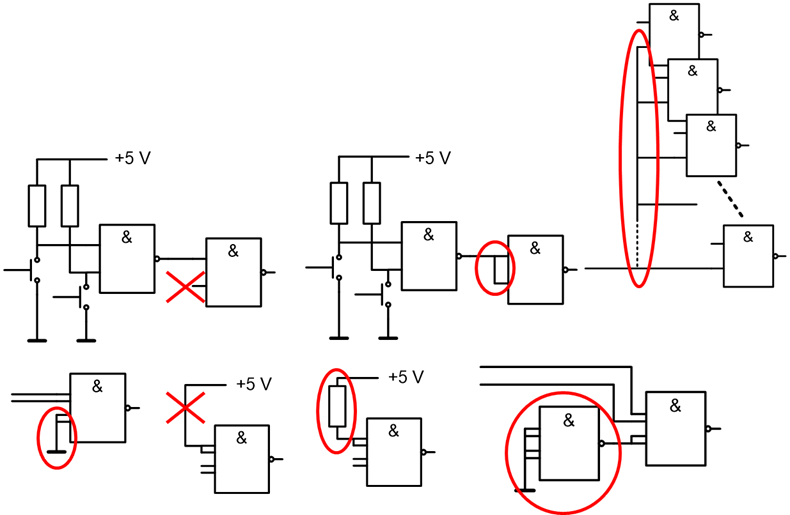
\includegraphics[width=0.9\textwidth]{fig/zapojovani.png}
		\end{center}
		
	\end{frame}
	
% =====================================================================================================================
	\begin{frame}
    \frametitle{Úrovně}
		
		\begin{itemize}
			\item Logická hradla různých technologií (TTL, HCTL, CMOS) mohou mít různá pásma vyhodnocení logické 0 a 1.
		\end{itemize}
		
		\begin{center}
			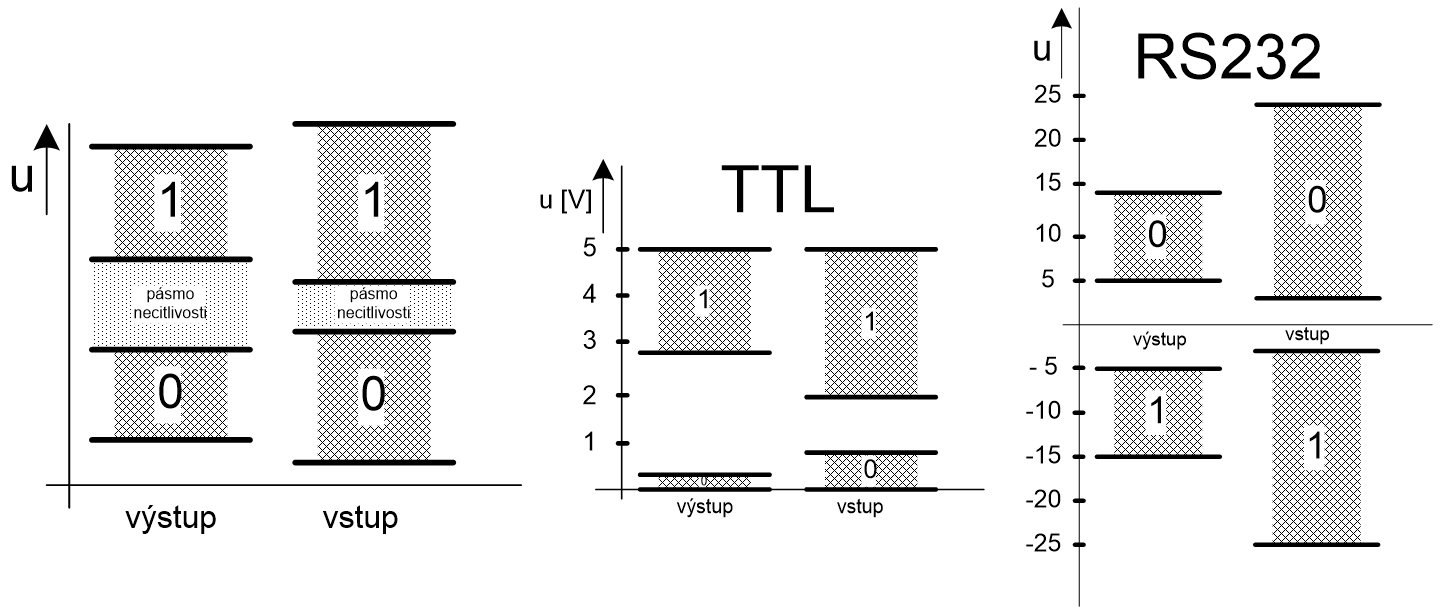
\includegraphics[width=\textwidth]{fig/pasma.png}
		\end{center}
		
	\end{frame}
	
% =====================================================================================================================
	\begin{frame}
    \frametitle{Zastupitelnost obvodů}
		\boldmath
		\begin{itemize}
			\item Úplnou logickou funkci lze získat:
			
			\begin{itemize}
				\item kombinací obvodů AND, OR, NEG,
				\item pouze obvody NAND,
				\item pouze obvody NOR.
			\end{itemize}
			
			\item Pokud jsou k dispozici jen hradla NAND (podobně pro NOR), upravujeme logickou funkci pomocí De Morganových zákonů.\\
			\vspace{3mm}
			\textbf{Příklad:} Získali jsme logickou funkci a potřebujeme, aby obsahovala jen součiny a negace:
			
			\begin{align*}
      Y =& \bar{A}B + BC +AB = \bar{\bar{Y}} = \\
				=& \overline{\overline{\bar{A}B + BC +AB}} \\
				=& \overline{\overline{\bar{A}B} \cdot \overline{BC} \cdot \overline{AB}} =
			\end{align*}
		\end{itemize}
		
	\end{frame}